%merke: $n^2$ oder n², aber nicht $$ und ² mischen

% ----- ab hier eigentlicher Inhalt -------------------------------------------

\section{Huffman-Codes}
\subsection*{}
\begin{frame}
	\frametitle{Aus der Vorlesung:}
	\begin{block}{Wozu Huffman Codes?}
    		\begin{itemize}
              \item Huffman-Codes komprimieren ein Wort $w \in A$* indem \pause
              \item häufigere Symbole durch kürzere Wörter \pause
              \item und seltener vorkommende Symbole durch längere Wörter kodiert werden
            \end{itemize}
    	\end{block}
\end{frame}

\begin{frame}{Huffman-Code}
	\begin{block}{Vorgehensweise}
		zwei Schritte:
    		\begin{enumerate}
			\item Konstruktion eines Baumes:
				\begin{itemize}
					\visible<2->{\item Blätter entsprechen $x \in A$}
					\visible<3->{\item Innere Knoten entsprechen Mengen von Symbolen}
					\visible<4->{\item An jedem Blatt wird das Symbol $x$ und dessen Häufigkeit notiert}
					\visible<5->{\item die zwei Elemente mit der geringsten Häufigkeit werden zu einem Elternknoten zusammengefasst}
				\end{itemize}
			\item Beschriftung der Kanten: links mit 0, rechts mit 1
		\end{enumerate}
		Der kürzeste Weg von der Wurzel zum Blatt gibt die Kodierung des jeweiligen Zeichens (im Blatt) an.
    	\end{block}
\end{frame}

\begin{frame}{Aufgabe}
	\begin{block}{Aufgabe 1}
    		Gegeben sei das Alphabet $X=\{a,b,c,d,e,f,g,h\}$.
    		\begin{enumerate}
			\item 1. Fall: Jedes Zeichen kommt genau einmal vor \\ Erstelle den Huffman-Code-Baum.\\
				\pause Wie lange wird die Kodierung von $w=badcfehg$? \pause
			\item 2. Fall: Zeichen a und b kommen zweimal, c viermal, d 8-mal, e 16-mal, f 32-mal, g 64-mal und h 128-mal vor. \\ Erstelle den Huffman-Code-Baum. Wie lange wird die Kodierung von $w=badcafehg$? \pause
			\item Wie lange wird ein Wort mit zweiter Zeichenverteilung, wenn man es mit dem ersten Code codiert?
			\item Wie lange wird ein Wort mit erster Zeichenverteilung, wenn man es mit dem zweiten Code codiert?
		\end{enumerate}
    	\end{block}

\end{frame}

\begin{frame}{Aufgabe}
	\begin{block}{Aufgabe 2}
    		Gegeben sei das Alphabet $X=\{a,b,c,d,e,f,g\}$ und die Auftrittswahrscheinlichkeiten $p(a)=\frac{3}{10}$, $p(b)=\frac{1}{10}$, $p(c)=\frac{1}{10}$, $p(d)=\frac{1}{7}$, $p(e)=\frac{1}{7}$, $p(f)=\frac{1}{7}$ und $p(g)=\frac{1}{14}$.
    		\begin{itemize}
			\item Erzeuge einen Huffman-Code C.
		\end{itemize}
    	\end{block}
	\visible<2->{
	\begin{block}{Lösung 2}
    		\begin{tabular}{cccccccc}
			Zeichen:&  a&    b&    c&    d&    e&    f&    g\\
			Wahrscheinlichkeit:&$\frac{3}{10}$&$\frac{1}{10}$&$\frac{1}{10}$&$\frac{1}{7}$&$\frac{1}{7}$&$\frac{1}{7}$&$\frac{1}{14}$ \\
			Code:&     00&  101&  110&  010&  011&  100&  111
		\end{tabular}
    	\end{block}
	}
\end{frame}

\begin{frame}{viele Codes}
	\begin{block}{mehrdeutig?}
    \begin{itemize}
      \item im Allgemeinen sind Huffman-Codes nicht indeutig:
		\item es können mehrere Zeichen gleichhäufig vorkommen
		\item Außerdem ist nicht festgelegt, welcher Knoten linker Nachfolger und welcher rechter Nachfolger eines inneren Knotens wird

		\item[$\Rightarrow$] Huffman-Codes sind nicht eindeutig
		\item Das macht aber nichts: alle, die sich für ein Wort $w$ ergeben können, sind "`gleich gut"'
	\end{itemize}
	\end{block}

\end{frame}


\section{Gerichtete Graphen}

\subsection*{}
\begin{frame}
	\frametitle{Motivation}

	\begin{block}{Gerichtete Graphen}
	\begin{itemize}
		\item \visible<1->{Einbahnstraßen}
		\item \visible<2->{Bahn- Flugverbindungen}
		\item \visible<3->{Stammbäume}
	\end{itemize}
	\end{block}

	\visible<4->{
	\begin{block}{Ungerichtete Graphen}
	\begin{itemize}
		\item Zweibahnstraßen
		\item \visible<5->{Irrgarten}
		\item \visible<6->{Stromnetz}
	\end{itemize}
	\end{block}}

	\visible<7->{
	\begin{block}{Nicht modellierbar}
		\begin{itemize}
			\item mehrspurige Verbindungen in gleicher Richtung
		\end{itemize}
	\end{block}}
\end{frame}

\begin{frame}
	\frametitle{Gerichteter Graph}
	\begin{block}{Definition}
	Ein gerichteter Graph $G$ ist ein Tupel $G=(V,E)$ mit
	\begin{itemize}
		\item der Grundmenge $V = \{v_i\}$ (die Menge der Ecken)
		\item der Relation $E\subseteq V\times V$ (die Menge der Kanten) \\ Notationen für Kanten:
		\begin{itemize}
			\item $(v,v')\in E$
			\item $v\rightarrow_G v'$
			\item $v \to v'$
		\end{itemize}
	\end{itemize}
	\end{block}
\end{frame}


\begin{frame}
	\frametitle{Zeichnerische Darstellung von gerichteten Graphen}

	\begin{block}{Ihr seid dran...}
		Ein kluger Ersti möchte gerne über die Weihnachtstage mit dem Zug nach Hause fahren. Um zu sehen über welche Strecken er alles fahren kann, malt er sich einen Graphen auf. \\ \pause
		Aus Aachen fahren Züge nach Berlin, Chemnitz und Dortmund. Während er von Berlin nur Chemnitz erreichen kann, gibt es Züge von Dortmund nach Chemnitz und Berlin. Essen ist leider von keiner dieser Städte erreichbar. \\
		Hinweis: Man malt die Ecken als Kreise und die Kanten als Pfeile.
	\end{block}
\end{frame}

\begin{frame}
	\begin{columns}
	\column{.5\textwidth}
		\begin{center}
		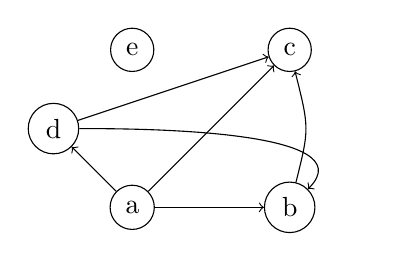
\begin{tikzpicture}
		  \tikzstyle{every node}=[draw,shape=circle];
			\path[fill] (0,0)  node[circle] (a) {a};
			\path[fill] (2,0)  node[circle] (b) {b};
			\path[fill] (2,2)  node[circle] (c) {c};
			\path[fill] (-1,1) node[circle] (d) {d};
			\path[fill] (0,2)  node[circle] (e) {e};

			\path[->,draw] (a) -- (b);
			\path[->,draw] (a) -- (d);
			\path[->,draw] (d) .. controls (0,1) and (3,1) .. (b);
			\path[->,draw] (b) .. controls (2.25,1) ..  (c);
			\path[->,draw] (a) -- (c);
			\path[->,draw] (d) -- (c);
		\end{tikzpicture}
		\end{center}
	\column{.5\textwidth}
		\begin{center}
		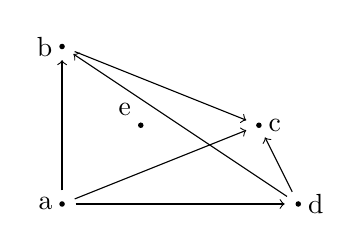
\begin{tikzpicture}
			\path[fill] (0,0)  node[circle] (a) {} node[left] {a} circle (1pt);
			\path[fill] (0,2)  node[circle] (b) {} node[left] {b} circle (1pt);
			\path[fill] (2.5,1)  node[circle] (c) {} node[right] {c} circle (1pt);
			\path[fill] (3,0) node[circle] (d) {} node[right] {d} circle (1pt);
			\path[fill] (1,1)  node[circle] (e) {} node[above left] {e} circle (1pt);

			\path[->,draw] (a) -- (b);
			\path[->,draw] (a) -- (d);
			\path[->,draw] (d) -- (b);
			\path[->,draw] (b) -- (c);
			\path[->,draw] (a) -- (c);
			\path[->,draw] (d) -- (c);
		\end{tikzpicture}
		\end{center}
	\end{columns}

	\vspace{1ex}
	\only<1>{Sind die beiden Graphen isomorph?}
	\only<2->{Ja, die beiden Graphen sind isomorph.}

	\vspace{2ex}
	\only<1>{Gebt die Graphen in Tupelschreibweise an!}
	\only<2>{Gebt den Graph in Tupelschreibweise an!}
	\only<3->{$G = ( \{a,b,c,d,e\}, \{(a,b),(a,c),(a,d),(b,c),(d,b),(d,c)\})$}
\end{frame}


\begin{frame}
	\frametitle{Graphen}
	\begin{block}{Begriffe}
		\begin{itemize}
			\item Ein Graph heißt \textbf{endlich}, wenn $V$ endlich ist ($|V|<\infty$).\pause
			\item 2 Knoten x und y heißen \textbf{adjazent}, wenn es eine Kante $(x,y)\in E$ gibt.\pause
			\item Eine \textbf{Schlinge} ist eine Kante der Form $(x,x)\in E$.\pause
			\item Ein Graph heißt \textbf{schlingenfrei}, wenn er keine Schlingen besitzt.\pause
			\item $G'=(V',E')$ ist ein \textbf{Teilgraph} von $G=(V,E)$, wenn $V'\subseteq V$ und $E'\subseteq E \cap V'\times V'$
		\end{itemize}
	\end{block}
\end{frame}

\begin{frame}
	\frametitle{Aufgabe}
	\begin{block}{Aufgabe}
		Gegeben sei ein gerichteter Graph mit n Knoten.
		\begin{itemize}
			\item Wieviele Kanten kann er maximal haben, wenn Schlingen erlaubt sind? \visible<2->{\textbf{Lösung:} n² Kanten}\pause
			\item Wieviele Kanten kann er maximal haben, wenn er schlingenfrei ist? \visible<3->{\textbf{Lösung:} $n(n-1)$ Kanten}
		\end{itemize}
	\end{block}
\end{frame}

\begin{frame}
	\frametitle{gerichtete Bäume}
	\begin{block}{Definition}
    In einem gerichteten Baum \ldots \pause
		\begin{itemize}
			\item  \ldots gibt es genau einen Knoten $r\in V$ so dass: \\
				für alle $x\in V$ ex. genau ein Pfad von $r$ nach $x$ \pause
			\item \ldots ist die Wurzel eindeutig
		\end{itemize}
	\end{block}
\end{frame}

\begin{frame}
	\frametitle{Pfade}
	\begin{block}{Definition}
		Ein Pfad ist eine nichtleere Liste $p=(v_0,\ldots ,v_n)\in V^+$, wenn für alle $i \in {\mathbb G}_n$ gilt $(v_i,v_{i+1})\in E$ \pause
		\begin{itemize}
			\item Die Anzahl $n=|p|-1$ (der Kanten!) heißt die \emph{Länge} des Pfades \pause
			\item Ein Pfad heißt \emph{wiederholungsfrei}, wenn alle Knoten $v_0,\ldots ,v_{n-1}$ und $v_1,\ldots ,v_n$ je paarweise verschieden sind, also maximal $v_0$ und $v_n$ gleich sind. \pause
			\item Falls $v_0=v_n$ heißt der Pfad \emph{geschlossen}. Dann ist der Pfad auch ein Zyklus.\pause
			\item ein geschlossener und wiederholungsfreier Pfad ist ein \emph{einfacher Zyklus}.
		\end{itemize}
	\end{block}
\end{frame}

\section{Ungerichtete Graphen}

\subsection*{}
\begin{frame}
	\frametitle{Ungerichteter Graph}
	\begin{block}{Definition}
		Ein ungerichteter Graph ist definiert als $U=(V,E)$, wobei
		\begin{itemize}
			\item $V = \{v_i\}$ die Menge der Ecken ist und
			\item $E\subseteq \{ \{x,y\}|x\in V \land y\in V\}$ die Menge der Kanten.
		\end{itemize}
	\end{block}

	\begin{center}
	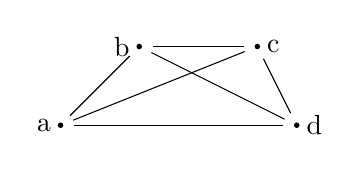
\begin{tikzpicture}
		\path[fill] (0,0)  node[circle] (a) {} node[left] {a} circle (1pt);
		\path[fill] (1,1)  node[circle] (b) {} node[left] {b} circle (1pt);
		\path[fill] (2.5,1)  node[circle] (c) {} node[right] {c} circle (1pt);
		\path[fill] (3,0) node[circle] (d) {} node[right] {d} circle (1pt);

		\path[draw] (a) -- (b);
		\path[draw] (a) -- (d);
		\path[draw] (d) -- (b);
		\path[draw] (b) -- (c);
		\path[draw] (a) -- (c);
		\path[draw] (d) -- (c);
	\end{tikzpicture}
	\\
	\vspace{1ex}
	\only<2->{Wie sähe dieser ungerichtete Graph als Menge aus?\\}
	\only<3->{$G = ( \{a,b,c,d\}, \{\{a,b\},\{a,c\},\{a,d\},\{b,c\},\{d,b\},\{d,c\}\})$}

	\end{center}
\end{frame}

\begin{frame}
	\frametitle{Aufgabe}
	\begin{block}{Aufgabe}
		Gegeben sei ein ungerichteter Graph mit n Knoten.
		\begin{itemize}
			\item Wieviele Kanten kann er maximal haben, wenn er schlingenfrei ist? \visible<2->{\textbf{Lösung:} $n(n-1)/2$ Kanten}\pause
			\item Wieviele Kanten kann er maximal haben, wenn Schlingen erlaubt sind? \visible<3->{\textbf{Lösung:} $n(n+1)/2$ Kanten}
		\end{itemize}
	\end{block}
\end{frame}

\begin{frame}
	\frametitle{zusammenhängende Graphen}
	\begin{block}{Definition}
    	Wir nennen \ldots
		\begin{itemize}
			\item einen gerichteten Graphen \emph{streng zusammenhängend},
				wenn für jedes Knotenpaar $(x,y)\in V^2$ gilt: Es gibt in $G$ einen Pfad von $x$ nach $y$.\\ \pause
			\item einen ungerichteten Graphen \emph{zusammenhängend}, wenn der entsprechende gerichtete Graph \emph{streng zusammenhängend} ist.
		\end{itemize}
	\end{block}
\end{frame}

\begin{frame}
	\frametitle{ungerichtete Bäume}
	\begin{block}{Definition}
		\begin{itemize}
			\item Jeder zusammenhängende ungerichtete Graph mit $|E| = |V| - 1$ ist ein ungerichteter Baum \pause
			\item Im ungerichteten Baum kann theoretisch jeder Knoten Wurzel sein. \\ \pause
			\item Daher wird i.d.R. ein Knoten als Wurzel hervorgehoben.
		\end{itemize}
	\end{block}
\end{frame}


\section{Abschluss}
% Studis anzuregen darüber nachzudenken, ob sie wirklich alles wissen, ansonsten nachlesen oder fragen nachträglich stellen, dann kann in der nächsten Woche nochmal drauf eingegangen werden
\subsection*{}
\begin{frame}
	\frametitle{Zum Schluss...}
	\begin{block}{Was ihr nun wissen solltet!}
	\begin{itemize}
		\visible<2->{\item Wie baue ich mir einen Huffman-Baum?}
		\visible<3->{\item Was ist ein Graph, was ein Teilgraph?}
		\visible<4->{\item Was bedeutet gerichtet, bzw. ungerichtet? }
		\visible<5->{\item Begriffe: Adjazent, Schlinge, Pfad, Zyklus, $\ldots$? }
	\end{itemize}
	\end{block}

	\visible<6->{
	\begin{block}{Ihr wisst was nicht?}
		Stellt \textbf{jetzt} Fragen!
	\end{block}}
\end{frame}
